\documentclass[aspectratio=169,t,11pt,table]{beamer}
\usepackage{../includes/slides,../includes/math}
\definecolor{accent}{HTML}{2B5269}
\definecolor{accent2}{HTML}{9D2235}

\title{Introduction to Linear Algebra}
\subtitle{\it  ECON 5753 — University of Arkansas}
\date{Sprint 2025}
\author{Prof. Kyle Butts}

\begin{document}

% ------------------------------------------------------------------------------
\begin{frame}[noframenumbering,plain]
\maketitle
\end{frame}
% ------------------------------------------------------------------------------

\section{Matrix Fundamentals}

\begin{frame}{Data}
  The basic currency of \emph{forecasting} is \alert{data}. Data typically looks like:

  \vspace*{2.5\bigskipamount}
  % head(mtcars[, c("mpg", "cyl", "hp", "wt", "am", "gear")]) |> tt() |> print("latex")
  \begin{table}
    \centering
    \begin{tabular}{cccccc}
      \toprule
      mpg & cyl & hp & wt & am & gear \\ \midrule %% TinyTableHeader
      21.0 & 6 & 110 & 2.620 & 1 & 4 \\
      21.0 & 6 & 110 & 2.875 & 1 & 4 \\
      22.8 & 4 &  93 & 2.320 & 1 & 4 \\
      21.4 & 6 & 110 & 3.215 & 0 & 3 \\
      18.7 & 8 & 175 & 3.440 & 0 & 3 \\
      \bottomrule
    \end{tabular}
  \end{table} 

  % \devgrid 
  \begin{tikzpicture}[remember picture, overlay]
    \node [anchor = east, text width = 0.2\textwidth] at (page cs:0.34,0.49) {
      \begin{center}
        \setstretch{0.8}
        {\footnotesize\color{raspberry} \emph{Rows} are observations $\rightarrow$}
      \end{center}
    };

    \node [anchor = south, text width = 0.2\textwidth] at (page cs:0.62,0.4) {
      \begin{center}
        \setstretch{0.8}
        {\footnotesize\color{purple} \emph{Columns} are variables $\downarrow$}
      \end{center}
    };
  \end{tikzpicture}
\end{frame}

\begin{frame}{Data as a matrix}
  The basic currency of \emph{linear algebra} are \alert{matrices}. Matrices look like this:
  
  $$
    \begin{bmatrix}
      21.0 & 6 & 110 & 2.620 & 1 & 4\\
      21.0 & 6 & 110 & 2.875 & 1 & 4\\
      22.8 & 4 &  93 & 2.320 & 1 & 4\\
      21.4 & 6 & 110 & 3.215 & 0 & 3\\
      18.7 & 8 & 175 & 3.440 & 0 & 3
    \end{bmatrix}
  $$ 
\end{frame}

\begin{frame}{Matrix notations}
  \vspace*{-\bigskipamount}
  $$
    \begin{bmatrix}
      21.0 & 6 & 110 & 2.620 & 1 & 4\\
      21.0 & 6 & 110 & 2.875 & 1 & 4\\
      22.8 & 4 &  93 & 2.320 & 1 & 4\\
      21.4 & 6 & 110 & 3.215 & 0 & 3\\
      18.7 & 8 & 175 & 3.440 & 0 & 3
    \end{bmatrix}
  $$ 

  \medskip
  Let's call this matrix, $\bm{A}$. Each element of $\bm{A}$ can be referred to as $A_{i,j}$ where $i$ is the \emph{row} and $j$ is the \emph{column}.
  \pause
  \begin{itemize}
    \item Unit $i$'s data is written $A_{i,\cdot}$
    \item Variable $j$ is written $A_{\cdot, j}$
  \end{itemize}
\end{frame}

\begin{frame}{Matrix Fundamentals}
  \begin{center}
    $\bm{A} = \begin{bmatrix}
        a_{11} & a_{12} & a_{13} \\
        a_{21} & a_{22} & a_{23} \\
      \end{bmatrix}$
  \end{center}

  The \alert{Size}/\alert{Dimension} a matrix: (rows) $\times$ (columns). E.g. $\bm{A}$ is a $2 \times 3$ matrix.
  \begin{itemize}
    \item The element in row $i$ and column $j$ is referred to as $a_{ij}$ or $A_{ij}$.
    
    \item A \alert{square matrix} is one with the same number of rows and columns. 
  \end{itemize}
\end{frame}

\begin{frame}{Vectors}
  A \alert{column vector}, often just ``vector'', is a $N \times 1$ matrix:
  $$
    v = \begin{bmatrix}v_1 \\ v_2 \\ \vdots \\ v_N\end{bmatrix}
  $$

  \bigskip
  In our previous discussion, each variable in a dataset can be thought of as a \emph{column vector}. A \emph{matrix}, then, is a collection of variables (vectors) glued together
\end{frame}


\begin{frame}{Matrix Addition and Subtraction}
  \begin{center}
    $A = \begin{bmatrix}
      {\color{orange} a_{11}} & {\color{orange} a_{12}} & {\color{orange} a_{13}} \\
      {\color{orange} a_{21}} & {\color{orange} a_{22}} & {\color{orange} a_{23}} \\
    \end{bmatrix}$ 
    and 
    $B = \begin{bmatrix}
      {\color{blue} b_{11}} & {\color{blue} b_{12}} & {\color{blue} b_{13}} \\
      {\color{blue} b_{21}} & {\color{blue} b_{22}} & {\color{blue} b_{23}} \\
    \end{bmatrix}$
  \end{center}

  \bigskip
  Dimensions must match: 
  $$
    ({\color{green} r} \times {\color{cranberry} c}) \pm ({\color{green} r} \times {\color{cranberry} c}) \implies ({\color{green} r} \times {\color{cranberry} c})
  $$

  \bigskip
  $A$ and $B$ are both $2 \times 3$ matrices, so we can add and subtract them: 
  $$
    A \pm B = \begin{bmatrix}
      {\color{orange} a_{11}} \pm {\color{blue} b_{11}} & {\color{orange} a_{12}} \pm {\color{blue} b_{12}} & {\color{orange} a_{13}} \pm {\color{blue} b_{13}} \\
      {\color{orange} a_{21}} \pm {\color{blue} b_{21}} & {\color{orange} a_{22}} \pm {\color{blue} b_{22}} & {\color{orange} a_{23}} \pm {\color{blue} b_{23}} \\
    \end{bmatrix}
  $$      
\end{frame}

\begin{frame}{Scalar Multiplication}
  \begin{center}
    $A = \begin{bmatrix}
      a_{11} & a_{12} & a_{13} \\
      a_{21} & a_{22} & a_{23} \\
    \end{bmatrix}$
  \end{center}

  For any scalar $c$ (a number like 2 or -4): 
  $$
    {\color{orange} c} A = \begin{bmatrix}
      {\color{orange} c} * a_{11} & {\color{orange} c} * a_{12} & {\color{orange} c} * a_{13} \\
      {\color{orange} c} * a_{21} & {\color{orange} c} * a_{22} & {\color{orange} c} * a_{23} \\
    \end{bmatrix}
  $$
\end{frame}

\begin{frame}{Scalar Multiplication}
  This is particularly useful when working with vectors, 
  $$
    {\color{orange} \beta} v = \begin{bmatrix}{\color{orange} \beta} v_1 \\ {\color{orange} \beta} v_2 \\ \vdots \\ {\color{orange} \beta} v_N\end{bmatrix}
  $$
\end{frame}

\begin{frame}{Regression as matrix operations}
  The most populate forecasting method we will learn is the \emph{linear regression}. Say we want to predict \texttt{mpg} given other variables about the car (\texttt{hp} and \texttt{wt}). 

  \bigskip
  To do so, we take variables, $A_{\cdot, j}$, and multiply it by their slope parameter to make predictions:

  $$
    \begin{bmatrix}1 \\ 1 \\ 1 \\ 1 \\ 1\end{bmatrix} \alpha + 
    \begin{bmatrix}110 \\ 110 \\ 93 \\ 110 \\ 175\end{bmatrix} \beta_{\texttt{hp}} + 
    \begin{bmatrix}2.620 \\ 2.875 \\ 2.320 \\ 3.215 \\ 3.440\end{bmatrix} \beta_{\texttt{wt}}
  $$
\end{frame}

\begin{frame}{Using matrices}
  The most populate forecasting method we will learn is the \emph{linear regression}. Say we want to predict \texttt{mpg} given other variables about the car (\texttt{hp} and \texttt{wt}). 
  
  \pause
  \bigskip
  To do so, we take variables, $A_{\cdot, j}$, and multiply it by their slope parameter to make predictions:

  $$
    \begin{bmatrix}1 \\ 1 \\ 1 \\ 1 \\ 1\end{bmatrix} \alpha + 
    \begin{bmatrix}110 \\ 110 \\ 93 \\ 110 \\ 175\end{bmatrix} \beta_{\texttt{hp}} + 
    \begin{bmatrix}2.620 \\ 2.875 \\ 2.320 \\ 3.215 \\ 3.440\end{bmatrix} \beta_{\texttt{wt}}
  $$
\end{frame}

\begin{frame}{Matrix multiplication}
  Using our rules of scalar multiplication and addition of vectors, we get:

  $$
    \begin{bmatrix}1 \\ 1 \\ 1 \\ 1 \\ 1\end{bmatrix} \alpha + 
    \begin{bmatrix}110 \\ 110 \\ 93 \\ 110 \\ 175\end{bmatrix} \beta_{\texttt{hp}} + 
    \begin{bmatrix}2.620 \\ 2.875 \\ 2.320 \\ 3.215 \\ 3.440\end{bmatrix} \beta_{\texttt{wt}} = 
    \begin{bmatrix}
      \alpha + 110 \beta_{\texttt{hp}} + 2.620 \beta_{\texttt{wt}} \\
      \alpha + 110 \beta_{\texttt{hp}} + 2.875 \beta_{\texttt{wt}} \\
      \alpha + \hphantom{0}93 \beta_{\texttt{hp}} + 2.320 \beta_{\texttt{wt}} \\
      \alpha + 110 \beta_{\texttt{hp}} + 3.215 \beta_{\texttt{wt}} \\
      \alpha + 175 \beta_{\texttt{hp}} + 3.440 \beta_{\texttt{wt}} 
    \end{bmatrix}
  $$

  \bigskip
  This is a \emph{linear combination} of the columns of the matrix
\end{frame}

\begin{frame}{Matrix Multiplication}
  \begin{center}
    $A = \begin{bmatrix}
        {\color{orange} a_{11}} & {\color{orange} a_{12}} & {\color{orange} a_{13}} \\
        {\color{cranberry} a_{21}} & {\color{cranberry} a_{22}} & {\color{cranberry} a_{23}} \\
    \end{bmatrix}$ 
    and 
    $D = \begin{bmatrix}
      {\color{blue} d_{11}} & {\color{green} d_{12}} \\
      {\color{blue} d_{21}} & {\color{green} d_{22}} \\
      {\color{blue} d_{31}} & {\color{green} d_{32}} \\
    \end{bmatrix}$
  \end{center}

  \bigskip
  Inner Dimensions must match: 
  $$
    ({\color{orange} r} \times \underline{\color{blue} c}) \times (\underline{\color{blue} c} \times {\color{green} p}) \implies ({\color{orange} r} \times {\color{green} p})
  $$

  \smallskip
  $A$ is a $2 \times 3$ and $D$ is a $3 \times 2$ matrix, so we can multiply (the 2s are equal): 
  \begin{center}
    $A \times D = \begin{bmatrix}
      {\color{orange} a_{11}} {\color{blue} d_{11}} + {\color{orange} a_{12}} {\color{blue} d_{21}} + {\color{orange} a_{13}} {\color{blue} d_{31}} & {\color{orange} a_{11}} {\color{green} d_{12}} + {\color{orange} a_{12}} {\color{green} d_{22}} + {\color{orange} a_{13}} {\color{green} d_{32}} \\

      {\color{cranberry} a_{11}} {\color{blue} d_{11}} + {\color{cranberry} a_{12}} {\color{blue} d_{21}} + {\color{cranberry} a_{13}} {\color{blue} d_{31}} & 
      {\color{cranberry} a_{11}} {\color{green} d_{12}} + {\color{cranberry} a_{12}} {\color{green} d_{22}} + {\color{cranberry} a_{13}} {\color{green} d_{32}} \\
    \end{bmatrix}$
  \end{center}
\end{frame}

\begin{frame}{Matrix Multiplication}
  \begin{center}
    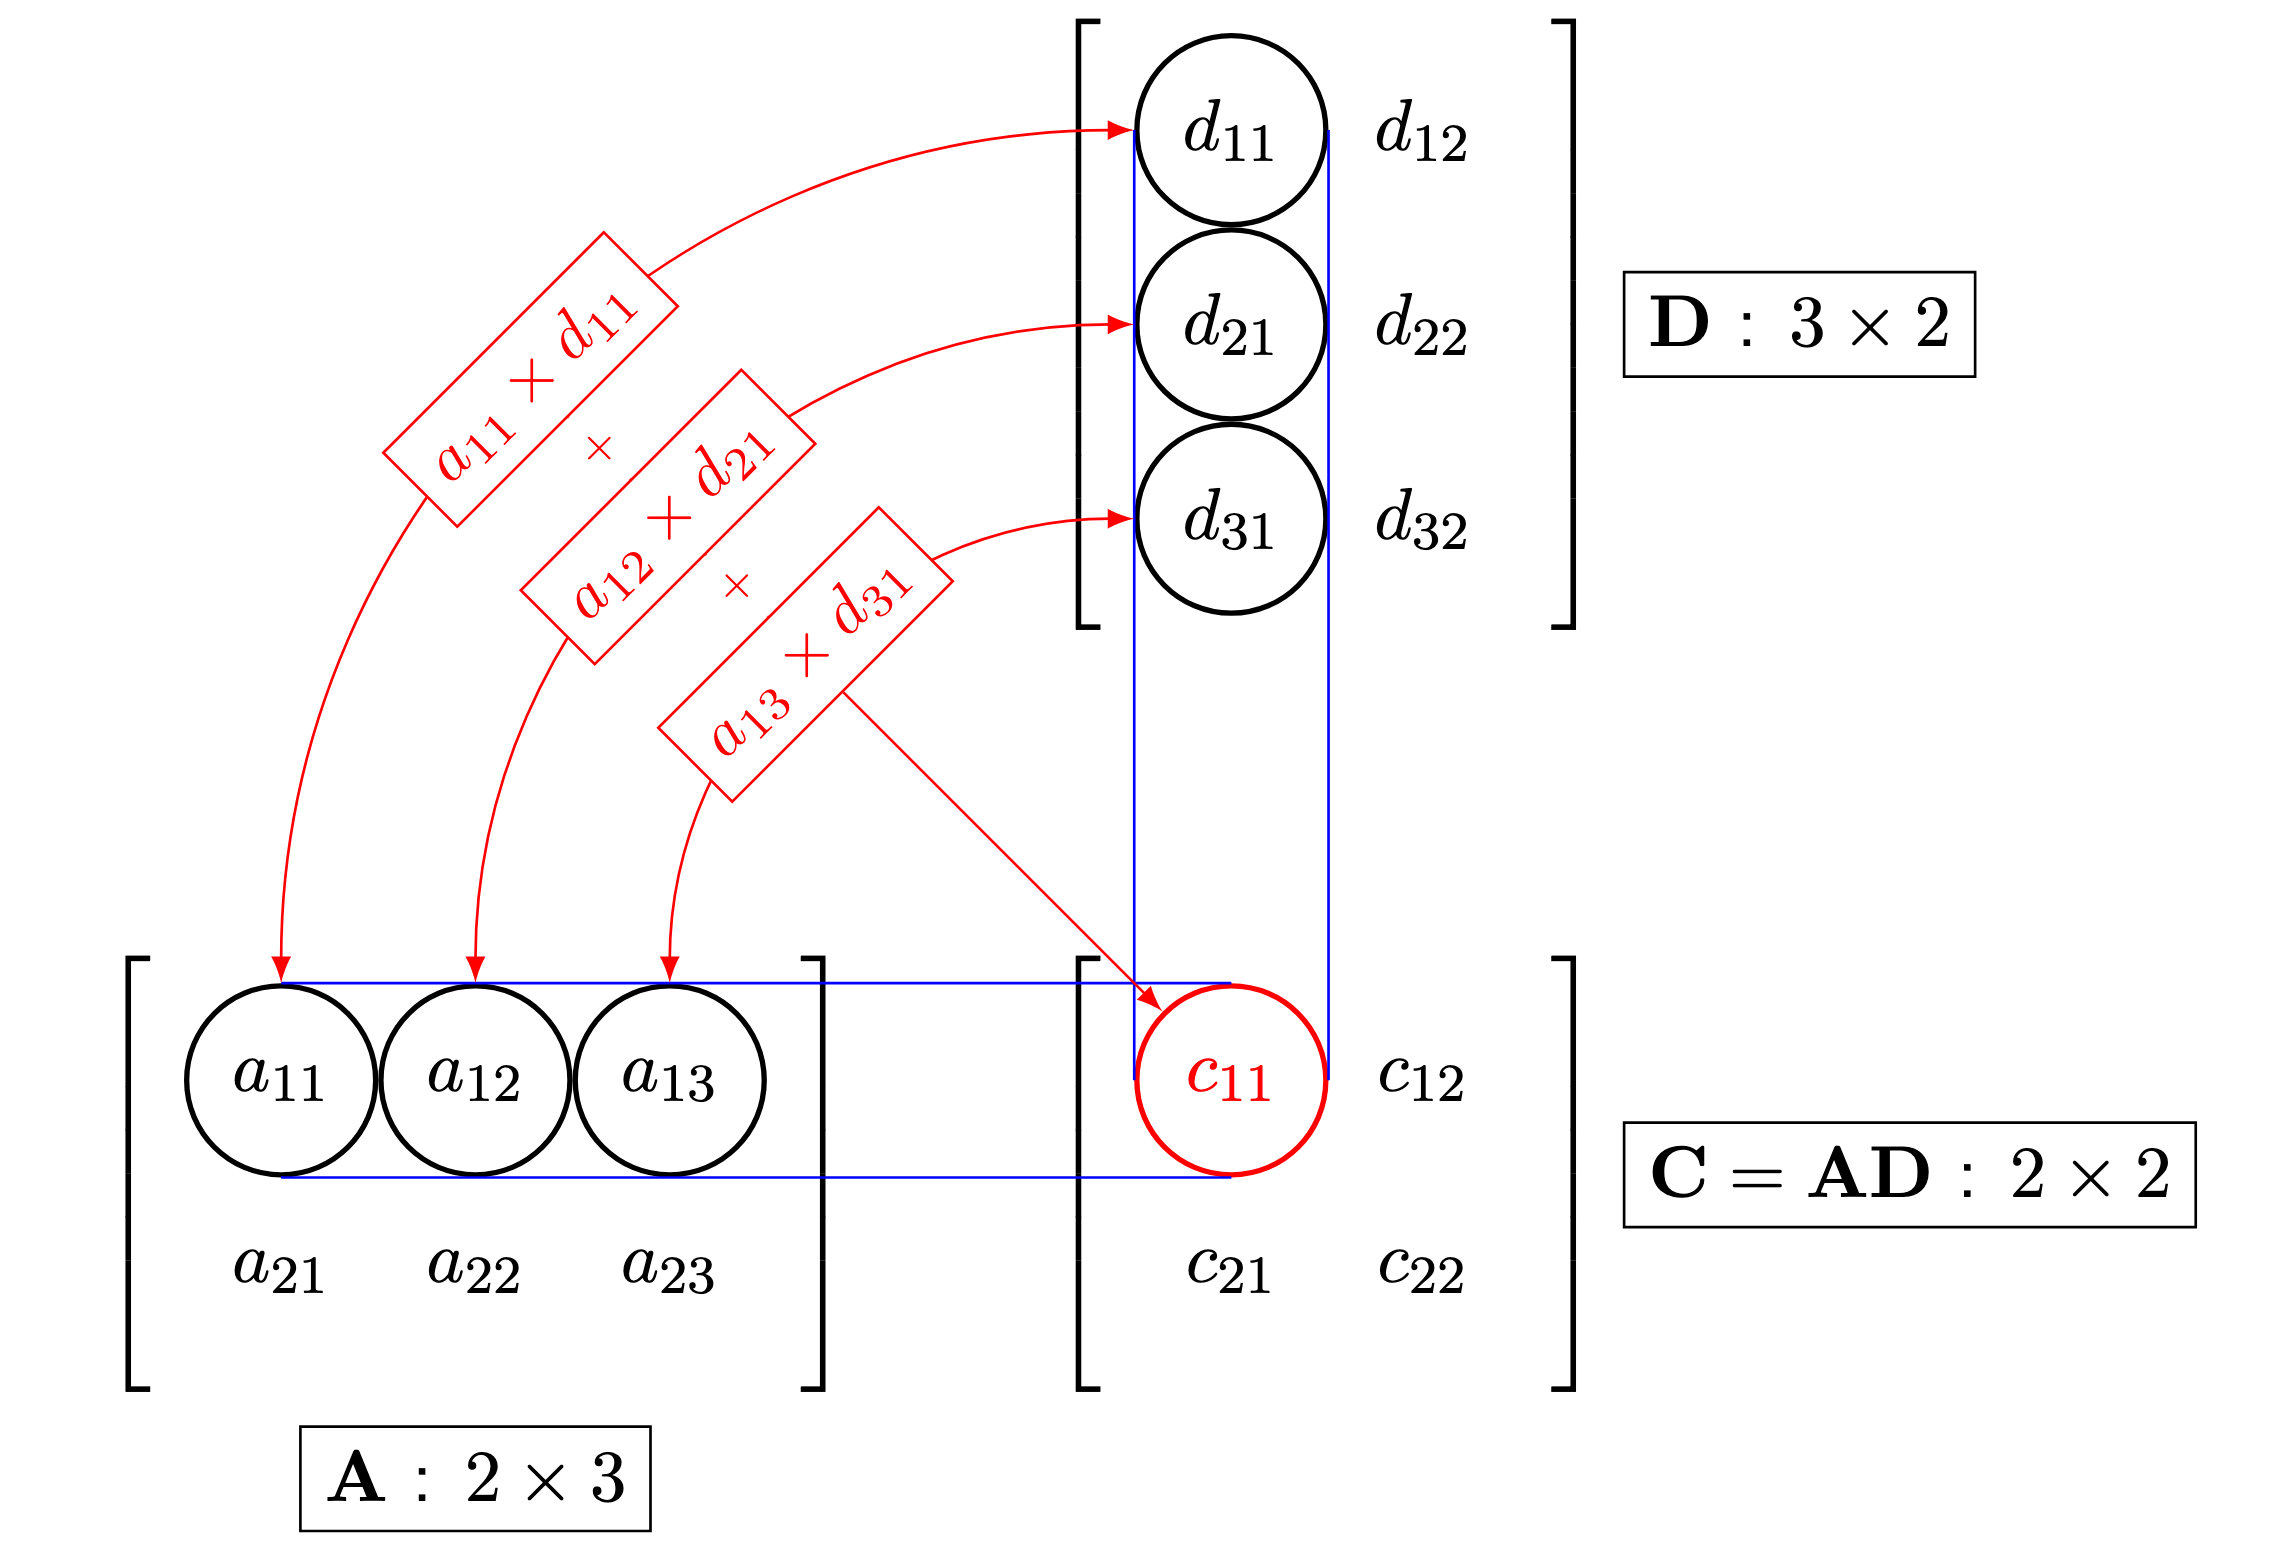
\includegraphics[width=0.65\textwidth]{figures/mat_mult.png}
  \end{center}
\end{frame}

\begin{frame}{Matrix Multiplication Practice}
  \begin{center}
    $A = \begin{bmatrix}
        1 & 4 & 1 \\
        2 & 3 & 2 \\
    \end{bmatrix}$ 
    and 
    $B = \begin{bmatrix}
      1 & 1 \\
      2 & 1 \\
      2 & 2 \\
    \end{bmatrix}$
  \end{center}

  \bigskip
  What is $A \times B$? What is $B \times A$?
\end{frame}

\begin{frame}{Matrix Multiplication in Regression}
  It turns out, we can write out our linear combination as a matrix times a vector
  $$
    \begin{bmatrix}
      1 & 110 & 2.620 \\ 
      1 & 110 & 2.875 \\ 
      1 & \hphantom{0}93 & 2.320 \\ 
      1 & 110 & 3.215 \\ 
      1 & 175 & 3.440
    \end{bmatrix}
    \begin{bmatrix}\alpha \\ \beta_{\texttt{hp}} \\ \beta_{\texttt{wt}}\end{bmatrix}
  $$

  \bigskip
  Verify that this product creates the same result
\end{frame}

\begin{frame}{Why call it ``multiplication''}
  There are two rules we learn about regular multiplication:
  \begin{enumerate}
    \item associative: $(ab)c = a(bc)$;
    \item distributive: $a (b + c) = ab + ac$; and 
    \item commutative: $ab = ba$
  \end{enumerate} 

  \pause
  \bigskip
  Matrices with multiplication and addition are associative, distributive, but \emph{NOT} commutative:
  \begin{enumerate}
    \item $(\bm{A} \bm{B}) \bm{C} = \bm{A} (\bm{B} \bm{C})$ 
    
    \item $\bm{A} (\bm{B} + \bm{C}) = \bm{A} \bm{B} + \bm{A} \bm{C}$
    
    \item However, $\bm{A} \bm{B} \neq \bm{A} \bm{B}$ (in some cases, this holds but not generally)
  \end{enumerate}
\end{frame}

\begin{frame}{Commutative}
  \vspace*{-\bigskipamount}
  $$\bm{A} \bm{B} \neq \bm{A} \bm{B}$$

  \bigskip
  In some cases, one of these two might not even exist. E.g.
  \begin{itemize}
    \item $\bm{A}$ is a $3 \times 2$ matrix and $\bm{B}$ is a $2 \times 1$ matrix.
  \end{itemize}

  $\bm{A} \bm{B}$ is well-defined (since the number of columns of $\bm{A} =$ the number of rows of $\bm{B}$), but $\bm{B} \bm{A}$ is not well-defined.
\end{frame}

\begin{frame}{Identity Matrix}
  In the same way that the number $1$ is special in multiplication of numbers (the `identity'), the \alert{identity matrix} takes the following form:
  $$
    \mathbb{I}_n = \begin{bmatrix} 
      1 & 0 & 0 & \dots & 0 \\
      0 & 1 & 0 & \dots & 0 \\
      0 & 0 & 1 & \dots & 0 \\
      \vdots & \vdots & \vdots & \ddots & \vdots \\ 
      0 & 0 & 0 & \dots & 1
    \end{bmatrix}
  $$

  \bigskip
  The identity matrix has the property that $\mathbb{I}_n \bm{A} = \bm{A} \mathbb{I}_n A = \bm{A}$
\end{frame}

\begin{frame}{Uses of Matrix Multiplication}
  Say I have some variable in my dataset $x$ and I want to know the sum of $x$ (or $1/n * $ the sum to get the sample mean). 

  \bigskip
  Take a few moments and try and think about what the matrix $\bm{S}$ would need to be to calculate the sample mean of $x$:
  $$
    \bm{S} \begin{bmatrix} x_1 \\ \vdots \\ x_n \end{bmatrix} = \frac{1}{n} \left( x_1 + \dots + x_n \right)
  $$
\end{frame}

\begin{frame}{Uses of Matrix Multiplication}
  \vspace*{-\bigskipamount}
  $$
    \begin{bmatrix} 1 & \dots & 1 \end{bmatrix} \begin{bmatrix} x_1 \\ \vdots \\ x_n \end{bmatrix} = \frac{1}{n} \left( x_1 + \dots + x_n \right)
  $$

  Answer: The \alert{row-vector} consisting of all $1$s 

  \pause
  \bigskip
  The column vector consisting of all 1s is often called ``iota'', $\iota = \begin{bmatrix}1 \\ \vdots \\ 1\end{bmatrix}$. 
  
  \smallskip
  The row vector is just $\iota$ flipped on it's side
\end{frame}

\begin{frame}{Transpose}
  The \alert{transpose} of a vector will do this ``flipping'' of vectors and matrices. We denote the transpose as $v^{\top}$ or $v'$
  \begin{itemize}
    \item The latter can be confused with `derivative', but is easier to write and arguably standard.
  \end{itemize}

  For vectors, the transpose is
  $$
    x = \begin{bmatrix} x_1 \\ \vdots \\ x_n \end{bmatrix} \iff x' = \begin{bmatrix} x_1 & \dots & x_n \end{bmatrix}
  $$
\end{frame}

\begin{frame}{Transpose}
  For matrices, the transpose is
  $$
    \bm{A} = \begin{bmatrix} A_{\cdot, 1} & \vdots & A_{\cdot, K} \end{bmatrix} \iff \bm{A}' = \begin{bmatrix} A_{\cdot, 1}' \\ \dots \\ A_{\cdot, K}' \end{bmatrix}
  $$

  \bigskip
  The $i$-th column of $\bm{A}$ becomes the $i$-th row of $\bm{A}'$
\end{frame}

\begin{frame}{Transpose rules}
  One rule worth knowing is $(ab)' = b' a'$

  \begin{itemize}
    \item I kind of remember it since transposing ``flips'' the rows and columns, you also flip the order of the vectors/matrices.
  \end{itemize}
\end{frame}

\begin{frame}{Sample mean}
  With this, we can write out sample mean more simply as 
  $$
    \bar{x} = \frac{1}{n} \iota' x
  $$
  
  Or, if we wanted the means of multiple varaibles, we could put them in a matrix and $$\frac{1}{n} \iota' \bm{X}$$ would be a row-vector of sample means
\end{frame}

\begin{frame}{Sample variance}
  Recall from your introductory statistics course, the sample variance of a variable is given by
  $$
    s^2 = \frac{1}{n-1} \sum_i (x_i - \bar{x})^2
  $$

  \bigskip
  Let $\tilde{x}_i \equiv x_i - \bar{x}$. For a minute, think about how you might calculate the sum of squares using the vector $\tilde{x}$
\end{frame}

\begin{frame}{Sample variance}
  \vspace*{-\bigskipamount}
  $$
    s^2 = \frac{1}{n-1} \tilde{x}' \tilde{x} = 
    \frac{1}{n-1} \begin{bmatrix}\tilde{x}_1 & \dots & \tilde{x}_n\end{bmatrix}
    \begin{bmatrix}\tilde{x}_1 \\ \vdots \\ \tilde{x}_n\end{bmatrix}
  $$
\end{frame}

\begin{frame}{Sample covariance}
  Similarly, we can write the covariance of two-variables as 
  $$
    \frac{1}{n-1} \tilde{x}' \tilde{y} = \frac{1}{n-1} \sum_i \tilde{x}_i \tilde{y}_i
  $$
\end{frame}

\begin{frame}{Variance Covariance Matrix}
  Consider a matrix of variable where each column is a (de-meaned) sample.
  $$
    \tilde{\bm{X}} = \begin{bmatrix}
      {\color{orange} x_1 - \bar{x}} & {\color{cranberry} y_1 - \bar{y}} & {\color{blue} z_1 - \bar{z}} \\
      {\color{orange} x_2 - \bar{x}} & {\color{cranberry} y_2 - \bar{y}} & {\color{blue} z_2 - \bar{z}} \\
      \vdots & \vdots & \vdots \\
      {\color{orange} x_n - \bar{x}} & {\color{cranberry} y_n - \bar{y}} & {\color{blue} z_n - \bar{z}} \\
    \end{bmatrix},
  $$ where $\bar{x}$ is the mean of variable $x$.
\end{frame}

\begin{frame}{Variance Covaraince Matrix}
  The Variance-Covariance Matrix is $\frac{1}{n-1} \tilde{\bm{X}}^T \tilde{\bm{X}}$

  $$
    = \frac{1}{n-1} 
    \begin{bmatrix}
      \sum_{i=1}^n {\color{orange} (x_i - \bar{x})}^2                                  & \sum_{i=1}^n {\color{orange} (x_i - \bar{x})}{\color{cranberry} (y_i - \bar{y})}  & \sum_{i=1}^n {\color{orange} (x_i - \bar{x})}{\color{blue} (z_i - \bar{z})}      \\
      \sum_{i=1}^n {\color{cranberry} (y_i - \bar{y})}{\color{orange} (x_i - \bar{x})} & \sum_{i=1}^n {\color{cranberry} (y_i - \bar{y})}^2                              & \sum_{i=1}^n {\color{cranberry} (y_i - \bar{y})}{\color{blue} (z_i - \bar{z})} \\
      \sum_{i=1}^n {\color{blue} (z_i - \bar{z})}{\color{orange} (x_i - \bar{x})}     & \sum_{i=1}^n {\color{blue} (z_i - \bar{z})}{\color{cranberry} (y_i - \bar{y})} & \sum_{i=1}^n {\color{blue} (z_i - \bar{z})}^2                                  \\
    \end{bmatrix}
  $$
  $$
    = \begin{bmatrix}
      Var({\color{orange} x})                       & Cov({\color{orange} x},{\color{cranberry} y})  & Cov({\color{orange} x},{\color{blue} z})      \\
      Cov({\color{cranberry} y},{\color{orange} x}) & Var({\color{cranberry} y})                   & Cov({\color{cranberry} y},{\color{blue} z}) \\
      Cov({\color{blue} z},{\color{orange} x})     & Cov({\color{blue} z},{\color{cranberry} y}) & Var({\color{blue} z})                       \\
    \end{bmatrix}
  $$
\end{frame}


\section{Matrix Transformations}

\begin{frame}{Matrix Times a Vector (Transformations)}
  $$
    A = \begin{bmatrix}
      {\color{orange} a_{11}} & {\color{green} a_{12}} \\
      {\color{blue} a_{21}} & {\color{cranberry} a_{22}}
    \end{bmatrix} 
    \text{ and } 
    x = \begin{bmatrix} x_1 \\ x_2 \end{bmatrix}
  $$

  An $n \times n$ matrix, $A$, times a $n \times 1$ vector, $x$, is a transformation from $\mathbb{R}^n$ to $\mathbb{R}^n$. So $A$ takes $x$, rotates it around and/or shrinks or extends the line.

  \pause
  \bigskip
  In general, 
  $$
    Ax = \begin{bmatrix}
      {\color{orange} a_{11}} x_1 + {\color{green} a_{12}} x_2\\
      {\color{blue} a_{21}} x_1 + {\color{cranberry} a_{22}} x_2
    \end{bmatrix} \in \mathbb{R}^2
  $$
\end{frame}

\begin{frame}{Transformation Examples}
  \only<1>{
    Our identity matrix, is a boring transformation:
    $$
      \begin{bmatrix} 1 & 0 \\ 0 & 1 \end{bmatrix}
      \begin{bmatrix} 2 \\ 3 \end{bmatrix} =
      \begin{bmatrix} 1*2 + 0*3 \\ 0*2 + 1*3 \end{bmatrix} =
      \begin{bmatrix} 2 \\ 3 \end{bmatrix}
    $$  
  }

  \only<2>{
  Reflection on the Y-axis: 
  $$
    \begin{bmatrix} -1 & 0 \\ 0 & 1\end{bmatrix} \begin{bmatrix} x \\ y \end{bmatrix} = \begin{bmatrix} -x \\ y \end{bmatrix}
  $$
  }

  \only<3>{
  Reflection  90 degrees clockwise: 
  $$
    \begin{bmatrix} 0 & 1 \\ -1 & 0\end{bmatrix} \begin{bmatrix} x \\ y \end{bmatrix} = \begin{bmatrix} y \\ -x \end{bmatrix}
  $$
  }

  \only<4>{
  Enlargement by scale factor $a$ in the $x$ direction and scale factor $b$ in the $y$ direction: 
  $$
    \begin{bmatrix} a & 0 \\ 0 & b \end{bmatrix} \begin{bmatrix} x \\ y \end{bmatrix} = \begin{bmatrix} ax \\ by \end{bmatrix}
  $$
  }
\end{frame}

\begin{frame}{Combination of Transformations}
  Let's say I want to rotate a vector 90 degrees clockwise and then keep only the $x$ direction (i.e. scale the $y$ by $0$.)
  \begin{itemize}
    \item I just multiply the matrices in the order I want to do them:
  \end{itemize}

  Let's try:
  $$
    \underbrace{\begin{bmatrix} 1 & 0 \\ 0 & 0 \end{bmatrix}}_{\text{Keep only } x} 
    \overbrace{\begin{bmatrix} 0 & 1 \\ -1 & 0 \end{bmatrix}}^{\text{Rotate 90 degrees clockwise}} 
    \begin{bmatrix} x \\ y \end{bmatrix} = 
    \pause
    \begin{bmatrix} 1 & 0 \\ 0 & 0 \end{bmatrix} \begin{bmatrix} y \\ -x \end{bmatrix} = \begin{bmatrix} y \\ 0 \end{bmatrix}
  $$
\end{frame}

\begin{frame}{Determinant of a Matrix}
  \begin{columns}[T]
    \begin{column}{.40\textwidth}
      When we rotate and scale an image, we are just doing many many vectors times a transformation matrix. 
      
      \medskip
      The \alert{determinant} asks how much does the area change with our transformation:
    \end{column}
    
    \hfill
    \begin{column}{.60\textwidth}
      
\includegraphics[width=\textwidth]{figures/determinant.png}
    \end{column}
  \end{columns}
\end{frame}

\begin{frame}{Formula for $2 \times 2$ Determinant}
  $$
    A = \begin{bmatrix}
      {\color{orange} a_{11}}  & {\color{green} a_{12}}     \\
      {\color{blue} a_{21}} & {\color{cranberry} a_{22}}
    \end{bmatrix}
  $$

  The \alert{Determinant} of $A$ is given by: 
  $$
    \mathrm{det}(A) = {\color{orange} a_{11}} * {\color{cranberry} a_{22}} - {\color{green} a_{12}} * {\color{blue} a_{21}}
  $$

  \begin{itemize}
    \item If $\mathrm{det}(A) = 1$, then the transformation preserves area

    \item If $\mathrm{det}(A)$ is greater than/smaller than $1$, then the transformation grows/shrinks area.

    \item If $\mathrm{det}(A) = 0$, then the transformation area shrinks to zero (you lose dimensions).
  \end{itemize}
\end{frame}

\section{Inverse of a Matrix}

\begin{frame}{Matrix Inverse}
  The final necessary linear algebra concept is that of the \alert{matrix inverse}. 
  \begin{itemize}
    \item It is equivalent to $1/x * x = 1$
  \end{itemize}

  \bigskip
  A \emph{square matrix} (i.e., dimension $n \times n$) $\bm{A}$ has an inverse $\bm{A}^{-1}$ if
  $$
    \bm{A}^{-1} \bm{A} = \mathbb{I}_n = \bm{A} \bm{A}^{-1}
  $$
\end{frame}

\begin{frame}{Inverse of Matrix}
  \vspace*{-\bigskipamount}
  $$
    \bm{A}^{-1} \bm{A} x = \mathbb{I}_n x = x
  $$
  
  The inverse of a matrix "undoes" the transformation done by $A$, i.e $A A^{-1} x = A^{-1} A x = x$.
  
  \pause
  \bigskip
  If the determinant of a matrix is 0, then the transformation does not have an inverse.   
  \begin{itemize}
    \item For example, the matrix that only keeps the $x$ component can't be inverted (what is the correct $y$ value?)
  \end{itemize}
\end{frame}

\begin{frame}{Inverse of 2x2 Matrix }
  $$
    A = \begin{bmatrix}
      {\color{orange} a_{11}}  & {\color{green} a_{12}} \\
      {\color{blue} a_{21}} & {\color{cranberry} a_{22}}
    \end{bmatrix}
  $$

  For $2x2$ matrices, there is a nice formula for the inverse: 
  $$
    \bm{A}^{-1} = 
    \underbrace{ \frac{1}{{\color{orange} a_{11}}  {\color{cranberry} a_{22}}  - {\color{green} a_{12}} {\color{blue} a_{21}} } }_{= \mathrm{det}(\bm{A})}
    \begin{bmatrix}
      {\color{cranberry} a_{22}} & - {\color{green} a_{12}} \\
      - {\color{blue} a_{21}}   & {\color{orange} a_{11}}
    \end{bmatrix}
  $$
\end{frame}

\begin{frame}{Inverse Example}
  $$
    \bm{A} = \begin{bmatrix} 2 & 4 \\ -4 & 10 \end{bmatrix}
  $$

  Find the inverse of $\bm{A}$ and verify it is indeed the inverse of $\bm{A}$
\end{frame}
\begin{frame}{Inverse Example}
  $$
    \bm{B} = \begin{bmatrix} 1 & 1 \\ 1 & 1 \end{bmatrix}
  $$

  What is the determinant of $\bm{B}$? Does $\bm{B}$ have an inverse?
\end{frame}



\section{Normal Random Variables}

\begin{frame}{Repeated Sampling}
  When conducting forecasts, we want to express uncertainty around our best guess, what is called \alert{statistical inference}.

  \bigskip
  We use the \alert{repeated sampling} framework to think about this:
  \begin{itemize}
    \item We collect one sample of data and estimate a model
    
    \item Imagine collecting \emph{many many} samples in the same way and estimating the model for each sample.
  \end{itemize}
\end{frame}  

\begin{frame}{Repeated Sampling and the Normal Distribution}
  In almost all cases, our estimates will be \alert{normally distributed} (at least in large samples).

  \bigskip
  For example, we know that the sample mean of a variable is approximately normally distributed:
  $$
    \bar{x} = \frac{1}{n} \sum_{i} x_i \sim \mathcal{N}(\mu, \frac{\sigma_x^2}{n})
  $$

  \pause
  \bigskip
  This allowed us to do things like:
  \begin{enumerate}
    \item Form confidence intervals, and
    
    \item Perform hypothesis tests
  \end{enumerate}
\end{frame}

\begin{frame}{Normal Distribution}
  We say a random variable is normally distributed and write it as 
  $$
    x \sim \mathcal{N}(\mu, \sigma^2),
  $$
  where $\mu = \expec{x}$ and $\sigma^2 = \var{x}$
\end{frame}

\imageframe{figures/ex_normal_dist.pdf}

\begin{frame}{Properties of Normal Distribution}
  We have $x \sim \mathcal{N}(\mu, \sigma^2)$. Say we perform some transformation of $x$:
  $$
    ax + b
  $$

  The modified variable is still normally distributed. Using properties of expectation and variance, we have:
  \begin{enumerate}
    \item $\expec{ax + b} = a\expec{x} + b = a\mu + b$
    
    \item $\var{ax + b} = \var{ax} = a^2 \var{x} = a^2 \sigma^2$
  \end{enumerate}


  \pause
  $$
    ax + b \sim \mathcal{N}\left(a\mu + b, a^2 \sigma^2\right)
  $$
\end{frame}

\begin{frame}{Random Vectors}
  We can extend this distribution to the \alert{joint distribution} of multiple random variables. Let $x = \begin{bmatrix}x_1 \\ \vdots \\ x_n \end{bmatrix}$ be a \alert{random vector}. 

  \bigskip
  These variables could be correlated with one another. For example, say $x_1$ is height and $x_2$ is weight of a surveyed person (or a sample mean of them).
  \begin{itemize}
    \item In repeated sampling, we expect $x_1$ and $x_2$ to be positively correlated. 
  \end{itemize}
\end{frame}

\begin{frame}{Expectation of Random Vector}
  \vspace*{-\bigskipamount}
  $$
    x = \begin{bmatrix}x_1 \\ \vdots \\ x_n \end{bmatrix}
  $$

  The expectation of the vector is just the expectation of each component variable
  $$
    \expec{x} = \begin{bmatrix} \expec{x_1} \\ \vdots \\ \expec{x_n} \end{bmatrix} = \begin{bmatrix} \mu_1 \\ \vdots \\ \mu_n \end{bmatrix}
  $$
\end{frame}

\begin{frame}{Covariance of Random Vector}
  \vspace*{-\bigskipamount}
  $$
    \tilde{x} = \begin{bmatrix} x_1 - \mu_1 \\ \vdots \\ x_n - \mu_n \end{bmatrix}
  $$  
  This vecotr has mean $0$. We can write the covariance of the random vector as

  $$
    \expec{\tilde{x} \tilde{x}'} = 
    \begin{bmatrix}
      \expec{(x_1 - \mu_1) (x_1 - \mu_1)} & \dots & \expec{(x_1 - \mu_1) (x_n \mu_n)} \\
      \vdots & \ddots & \vdots \\
      \expec{(x_n - \mu_n) (x_1 - \mu_1)} & \dots & \expec{(x_n - \mu_n) (x_n \mu_n)} \\
    \end{bmatrix}
  $$
\end{frame}

\begin{frame}{Covariance of Random Vector}
  From the previous slide, we have
  $$
    \Sigma \equiv \expec{(x-\mu) (x-\mu)'} = 
    \begin{bmatrix}
      \var{x_1} & \dots & \cov{x_1, x_n} \\
      \vdots & \ddots & \vdots \\
      \cov{x_n, x_1} & \dots & \var{x_n} \\
    \end{bmatrix}
  $$

  The diagonal of this matrix is the variance of each variable. The off-diagonal elements are the covariance between the varaibles.
  \pause
  \begin{itemize}
    \item If the off-diagonal element are all $0$, then the random variables are uncorrelated.
  \end{itemize}
\end{frame}

\begin{frame}{Multivariate Normal Distribution}
  In particular, we might estimate a few parameters in our model and they will each be normally distributed. 

  \bigskip
  But, even stronger, these estimates (a random vector) $x$ are multivariate normally distributed:
  $$
    x = \begin{bmatrix}x_1 \\ \vdots \\ x_n \end{bmatrix} \sim 
    \mathcal{N}\left( \mu, \Sigma \right)
  $$
  where $\Sigma \equiv \expec{(x-\mu) (x-\mu)'}$
\end{frame}

\imageframe{figures/mvnorm_heatmap_independent.pdf}
\imageframe{figures/mvnorm_heatmap_weak_pos_corr.pdf}
\imageframe{figures/mvnorm_heatmap_strong_neg_corr.pdf}

\begin{frame}{Linear combinations of multivariate random variable}
  Say $x \sim \mathcal{N}\left( \mu, \Sigma \right)$ and $a = \begin{bmatrix}a_1 \\ \vdots \\ a_n\end{bmatrix}$
  
  Then, the product $a' x$ is a linear combination of $x_i$ and is normally distributed:
  $$
    a'x = \sum_i a_i x_i \sim \mathcal{N}(?, ?)
  $$
\end{frame}

\begin{frame}{Linear combinations of multivariate random variable}
  Say $x \sim \mathcal{N}\left( \mu, \Sigma \right)$ and $a = \begin{bmatrix}a_1 \\ \vdots \\ a_n\end{bmatrix}$

  \bigskip
  First, consider the expectation of $a'x$
  \begin{align*}
    \expec{a'x} = \expec{\sum_i a_i x_i} &= \sum_i a_i \expec{x_i} \\
    &= \sum_i a_i \mu_i \\
    &= a' \mu
  \end{align*}
\end{frame}

\begin{frame}{Linear combinations of multivariate random variable}
  Second, consider the variance of $a'x$
  \begin{align*}
    \var{a'x} &= \expec{(a'x - a'\mu) (a'x - a'\mu)'} \\
    &= \expec{(a'(x - \mu)) (a'(x - \mu))'} \\
    \pause
    &= \expec{a' (x - \mu) (x - \mu)' a} = a' \Sigma a
  \end{align*}

  \pause
  \bigskip
  Therefore, if $x \sim \mathcal{N}\left( \mu, \Sigma \right)$, then
  $$
    a'x = \sum_i a_i x_i \sim \mathcal{N}(a'\mu, a'\Sigma a)
  $$
\end{frame}

\section{Derivatives of matrix expressions}

\begin{frame}{Derivatives}
  If you recall, we had the following definition of a derivative:
  $$
    \frac{d}{dx} f(x) = \lim_{h \to 0} \frac{f(x + h) - f(x)}{h}
  $$

  \bigskip
  You could write this as an approximation:
  $$
    f(x + dx) - f(x) \approx \frac{d}{dx} f(x) * dx
  $$
  In words, the change in $f$ is approximately equal to  the derivative times the change in $x$
  % \bigskip
  % You were always told you can not "multiply"  by the $dx$. 
\end{frame}

\imageframe{figures/differential_as_linear_approximation.jpg}

\begin{frame}{Taylor Expansion}
  This formulation is actually the basis of the Taylor Expansion that you may have learned in your calculus course:
  $$
    f(x + dx) \approx f(x) + \frac{d}{dx} f(x) * dx + \text{\footnotesize something small}
  $$  
  
  \begin{itemize}
    \item So long as $dx$ is ``small'', this approximation is quite accurate.
  \end{itemize}
\end{frame}

\begin{frame}{Multivariate derivative}
  Say $f$ is now a function that takes a vector $x$ ($\mathbb{R}^n$) and produces a scalar output ($\mathbb{R}$). How $f$ changes depends on which of the input $x_i$ you are changing.

  $$
    \frac{\partial}{\partial x}  f(x) \equiv \begin{bmatrix}
      \frac{\partial}{\partial x_1} f(x) \\ \vdots \\ \frac{\partial}{\partial x_n} f(x)
    \end{bmatrix}
  $$

  \bigskip
  This is called the ``gradient'' and it is a vector containing the partial derivatives
\end{frame}

\begin{frame}{Multivariate derivative}
  Our linear approximation holds in this setting to. Let $dx$ be the column vector of changes in each $x_i$: $dx = \begin{bmatrix}dx_1 & \dots & dx_n\end{bmatrix}'$.

  \pause
  \bigskip
  Then our approximation is as follows:
  \begin{align*}
    f(x + dx)  &\approx f(x) + \frac{\partial}{\partial x} f(x)' dx \\
    &= 
    f(x) +
    \begin{bmatrix} \frac{\partial}{\partial x_1} f(x) & \dots & \frac{\partial}{\partial x_n} f(x) \end{bmatrix} 
    \begin{bmatrix}dx_1 \\ \vdots \\ dx_n\end{bmatrix} \\ 
    \pause
    &= f(x) + \sum_i \frac{\partial f(x)}{\partial x_i} dx_i
  \end{align*}
\end{frame}

% Helpful: https://bookdown.org/compfinezbook/introcompfinr/Derivatives-of-Simple-Matrix-Functions.html
\begin{frame}{Useful matrix derivative rules}
  Let $x$ and $y$ be vectors of the same length. The derivative of the dot product $x' y$ can be given as
  $$
    \frac{\partial}{\partial x} x' y = y
  $$

  and 
  $$
    \frac{\partial}{\partial y} x' y = x
  $$
\end{frame}

\begin{frame}{Useful matrix derivative rules}
  Let $\bm{A}$ be a matrix and $x$ a vector.
  $$
    \frac{\partial}{\partial x} \bm{A}x = \bm{A}
  $$

  More, using the \emph{chain rule} for derivatives, you could show
  $$
    \frac{\partial}{\partial x} x'\bm{A}x = 2\bm{A}x
  $$
  
  \bigskip
  You can see the proofs here: \url{https://bookdown.org/compfinezbook/introcompfinr/Derivatives-of-Simple-Matrix-Functions.html}
\end{frame}

\end{document}
